%
%%%%%%%%%%%%%%%%%%%%%%%%%%%%%%%%%%%%%%%%%%%%%%%%%%
% PLANTILLA EJERCICIOS DE HISTORIA DE LA MÚSICA I
% Este es un modelo para redactar los ejercicios
% 
% Pasos para cubrir la plantilla:
% 1) Realizar una copia de este modelo
% 2) Renombrar el archivo:
%		"HM1_Hoja(número).tex"
% 3) El número de Hoja debe ser correlativo
% 
%%%%%%%%%%%%%%%%%%%%%%%%%%%%%%%%%%%%%%%%%%%%%%%%%%
%
% Esta plantilla es para crear ejercicios de esta materia
% Se recomienda crear un archivo por cada tema
% Descomentar según se necesite utilizar un modelo de ejercicio u otro
% Clase de documento:
\documentclass[letterpaper,12pt,notitlepage,spanish]{article}
%
% Archivo externo de configuración
% --------------------------------
% Seleccionar o idioma:
%%%%%%%%%%%%%%%%%%%%%%%%%%%%%%%%%%%%%%%%%%%
%% ---------- MODELO EJERCICIOS ---------- 
%% MATERIA: HISTORIA
%% CURSO: 
%% AÑO ACADÉMICO: 
%% CENTRO: 
%%%%%%%%%%%%%%%%%%%%%%%%%%%%%%%%%%%%%%%%%%%
%% 
%% MODELO PARA REDACTAR EJERCICIOS
%% ===============================
%% 
%% Clase de documento
%% ------------------
%\documentclass[letterpaper,12pt,notitlepage,spanish]{article}
%\documentclass[12pt,a4paper,notitlepage]{article}
%
% Márgenes de documento
% ---------------------
\usepackage[left=2.0cm, right=2.0cm, lines=45, top=2.5cm, bottom=2.0cm]{geometry}
%
% Paquetes necesarios
% -------------------
\usepackage[utf8]{inputenc} % acentos en ES
\usepackage[spanish,activeacute, es-tabla]{babel}
\usepackage{enumerate} % entornos de listas
\usepackage{multicol}  % varias columnas texto
\usepackage{fancyhdr}  % encabezado personalizado
\usepackage{fancybox}  % entornos con cajas
\usepackage{pdfpages}  % páginas pdf
%\usepackage[none]{hyphenat} % evitar separación silábica
%
\usepackage{lipsum} % generar texto aleatorio "loren ipsum"
\usepackage{environ} 
\usepackage{probsoln} % paquete para soluciones
%\showanswers % para mostrar soluciones
%
%Esto es lo importante. Ponemos la solución al margen.
\NewEnviron{solutionnew}{%
%  \leavevmode\marginpar{\raggedright\footnotesize \textbf{Solución:}\\ \BODY}
%  \textbf{Solución:}\\ \BODY} % sol. con salto de liña
  \small{Solución:} \BODY} % sol. na mesma liña
  {}
\renewenvironment{solution}{\solutionnew}{\endsolutionnew}
%
% FIGURAS EN COLUMNAS:
\newenvironment{Figura}
  {\par\medskip\noindent\minipage{\linewidth}}
  {\endminipage\par\medskip}
% ---
%
% Lineas de encabezado y pié
% --------------------------
\renewcommand{\headrulewidth}{0.5pt}
%\renewcommand{\headrulewidth}{1.0pt}
\renewcommand{\footrulewidth}{0.5pt}
%\renewcommand{\footrulewidth}{1.0pt}
\pagestyle{fancy} % estilo de página
%
% Recuadros y figuras
% -------------------
\newcommand\Loadedframemethod{TikZ}
\usepackage[framemethod=\Loadedframemethod]{mdframed}
\usepackage{tikz}
\usetikzlibrary{calc,through,backgrounds}
\usetikzlibrary{matrix,positioning}
%Desssins geometriques
\usetikzlibrary{arrows}
\usetikzlibrary{shapes.geometric}
\usetikzlibrary{datavisualization}
\usetikzlibrary{automata} % LATEX and plain TEX
\usetikzlibrary{shapes.multipart}
\usetikzlibrary{decorations.pathmorphing} 
\usepackage{pgfplots}
\usepackage{physics}
\usepackage{titletoc}
\usepackage{mathpazo} 
\usepackage{algpseudocode}
\usepackage{algorithmicx} 
\usepackage{bohr} 
\usepackage{xlop} 
\usepackage{bbding} 
%\usepackage{minibox} 
% Texto árabe
\usepackage{mathdesign}
\usepackage{bbding} 
% --
% --
%   ---------   Personalización de textos    ---------
%   Opción en Galego.-
\addto\captionsspanish{
\renewcommand{\contentsname}{Índice} 
\renewcommand{\listfigurename}{Índice de ilustracións} 
\renewcommand{\listtablename}{Índice de táboas} 
\renewcommand{\bibname}{Bibliografía} 
\renewcommand{\indexname}{Indice alfabético} 
\renewcommand{\figurename}{Ilustración} 
\renewcommand{\tablename}{Táboa} 
%\renewcommand{\appendixname}{Anexo} 
%\renewcommand{\abstractname}{Resumo}
%\renewcommand{\partname}{BLOQUE} % Cambio Parte BLOQUE
%\renewcommand{\chaptername}{TEMA} % Cambio CAPÍTULO por TEMA en mayúsculas %
}
%   ---------   Fin personalización de textos   ---------

% Tipograía:
% ----------
% Fuente HEURÍSTICA (cómoda de leer)
%\usepackage{heuristica}
% Fuente LIBERTINE (cómoda para apuntes)
\usepackage{libertineRoman}
%\usepackage[proportional]{libertine}
% Fuente ROMANDE (estilo antiguo pero no muy cómoda)
%\usepackage{romande} %
% 
% Encabezado y pié de página (textos)
% -----------------------------------
% Modelo 1:
% ---------
% texto de encabezado izquierda:
%\lhead{\normalfont{Historia de la Música I}}
% texto encabezado centro:
%\chead{\textbf{Ejercicios}}
% texto de encabezado derecha:
%\rhead{\normalfont{curso: 2020/2021}}
% texto pié izquierdo:
%\lfoot{\small{\textit{}}}
% texto pié centrado:
%\cfoot{\textsc{Pág. \thepage }}
% texto pié derecho
%\rfoot{\textit{Pr. $\mathcal{A}$.Kaal}}
% ----------
% Modelo 2:
% ---------
% Encabezado y pié de página (textos)
% -----------------------------------
% texto de encabezado izquierda:
%
%\lhead{
%	\hrule
%	\vspace*{0.20cm}
%	\normalfont{Historia de la Música I}
%	\vspace*{0.10cm}
	%\hrule
%}
% texto encabezado centro:
%\chead{
%	\textbf{Cuestionario de Ejercicios}
%	\vspace*{0.08cm}}
% texto de encabezado derecha:
%\rhead{
%	\normalfont{curso: 2020/2021}
%	\vspace*{0.08cm}}
%
% texto pié izquierdo:
%\lfoot{
	%\begin{center}
		%\vspace*{0.20cm}
		%\hrule
		%\small{
		%Conservatorio Profesional de Música de Viveiro - Avda. da mariña s/n - (27850) Viveiro - Lugo
		%	}
	%\end{center}
%}
% texto pié centrado:
%\cfoot{
	%\vspace*{0.30cm}
	%\hrule
	%\vspace*{0.90cm}
%	\small{- Página \thepage -  }\\
	%\small{Conservatorio Profesional de Música de Viveiro}\\
	%\small{avda. da Mariña s/n}
%}

% ----------
% Modelo 3:
% ---------
% Encabezado y pié de página (textos)
% -----------------------------------
% texto de encabezado izquierda:
%
\lhead{
	\hrule
	\vspace*{0.20cm}
	\normalfont{Historia da Música I}
	\vspace*{0.10cm}
	%\hrule
}
% texto encabezado centro:
\chead{
	\textbf{CADERNO DE EXERCICIOS}
	\vspace*{0.08cm}}
% texto de encabezado derecha:
\rhead{
	\normalfont{curso: 2022/2023}
	\vspace*{0.08cm}}
%
% texto pié izquierdo:
%\lfoot{
%	\begin{center}
%		\vspace*{0.20cm}
%		\hrule
%		\small{
%		Conservatorio Profesional de Música de Viveiro - Avda. da mariña s/n - (27850) Viveiro - Lugo
%			}
%	\end{center}
%}
% texto pié centrado:
\cfoot{
	%\vspace*{0.30cm}
	%\hrule
	%\vspace*{0.90cm}
	\small{- \thepage -  }\\
	%\small{Conservatorio Profesional de Música de Viveiro}\\
	%\small{avda. da Mariña s/n}
}

% --------
%=====================Algo setup
\algblock{If}{EndIf}
\algcblock[If]{If}{ElsIf}{EndIf}
\algcblock{If}{Else}{EndIf}
\algrenewtext{If}{\textbf{si}}
\algrenewtext{Else}{\textbf{sinon}}
\algrenewtext{EndIf}{\textbf{finsi}}
\algrenewtext{Then}{\textbf{alors}}
\algrenewtext{While}{\textbf{tant que}}
\algrenewtext{EndWhile}{\textbf{fin tant que}}
\algrenewtext{Repeat}{\textbf{r\'ep\'eter}}
\algrenewtext{Until}{\textbf{jusqu'\`a}}
\algcblockdefx[Strange]{If}{Eeee}{Oooo}
[1]{\textbf{Eeee} "#1"}
{\textbf{Wuuuups\dots}}

\algrenewcommand\algorithmicwhile{\textbf{TantQue}}
\algrenewcommand\algorithmicdo{\textbf{Faire}}
\algrenewcommand\algorithmicend{\textbf{Fin}}
\algrenewcommand\algorithmicrequire{\textbf{Variables}}
\algrenewcommand\algorithmicensure{\textbf{Constante}}% replace ensure by constante
\algblock[block]{Begin}{End}
\newcommand\algo[1]{\textbf{algorithme} #1;}
\newcommand\vars{\textbf{variables } }
\newcommand\consts{\textbf{constantes}}
\algrenewtext{Begin}{\textbf{debut}}
\algrenewtext{End}{\textbf{fin}}
%================================
%================================

\setlength{\parskip}{1.25cm}
\setlength{\parindent}{1.25cm}
\tikzstyle{titregris} =
[draw=gray,fill=gray, shading = exersicetitle, %
text=gray, rectangle, rounded corners, right,minimum height=.3cm]
\pgfdeclarehorizontalshading{exersicebackground}{100bp}
{color(0bp)=(green!40); color(100bp)=(black!5)}
\pgfdeclarehorizontalshading{exersicetitle}{100bp}
{color(0bp)=(red!40);color(100bp)=(black!5)}
\newcounter{exercise}
%\renewcommand*\theexercise{exercice \textbf{Ejercicio}~n\arabic{exercise}} % CASTELÁN
\renewcommand*\theexercise{exercice \textbf{Exercicio}~n\arabic{exercise}} % GALEGO
\makeatletter
\def\mdf@@exercisepoints{}%new mdframed key:
\define@key{mdf}{exercisepoints}{%
\def\mdf@@exercisepoints{#1}
}
\mdfdefinestyle{exercisestyle}{%
outerlinewidth=1em,outerlinecolor=white,%
leftmargin=-1em,rightmargin=-1em,%
middlelinewidth=0.5pt,roundcorner=3pt,linecolor=black,
apptotikzsetting={\tikzset{mdfbackground/.append style ={%
shading = exersicebackground}}},
innertopmargin=0.1\baselineskip,
skipabove={\dimexpr0.1\baselineskip+0\topskip\relax},
skipbelow={-0.1em},
needspace=0.5\baselineskip,
frametitlefont=\sffamily\bfseries,
settings={\global\stepcounter{exercise}},
singleextra={%
\node[titregris,xshift=0.5cm] at (P-|O) %
{~\mdf@frametitlefont{\theexercise}~};
\ifdefempty{\mdf@@exercisepoints}%
{}%
{\node[titregris,left,xshift=-1cm] at (P)%
{~\mdf@frametitlefont{\mdf@@exercisepoints points}~};}%
},
firstextra={%
\node[titregris,xshift=1cm] at (P-|O) %
{~\mdf@frametitlefont{\theexercise}~};
\ifdefempty{\mdf@@exercisepoints}%
{}%
{\node[titregris,left,xshift=-1cm] at (P)%
{~\mdf@frametitlefont{\mdf@@exercisepoints points}~};}%
},
}
\makeatother

%%%%%%%%%%%%%%%5 Definición modificada %%%%%%%%%%%%%%%%%%%%%%%%%
%
% Modificado para traballar con banco de exercicios
% Elimino as liñas do recadro de exercicios convencional
%
%\mdfdefinestyle{theoremstyle}{%
%outerlinewidth=0.01em,linecolor=white,middlelinewidth=0.5pt,%
%frametitlerule=true,roundcorner=2pt,%
%apptotikzsetting={\tikzset{mfframetitlebackground/.append style={%
%shade,left color=white, right color=blue!20}}},
%frametitlerulecolor=white,innertopmargin=1\baselineskip,%green!60,
%innerbottommargin=0.5\baselineskip,
%frametitlerulewidth=0.1pt,
%innertopmargin=0.7\topskip,skipabove={\dimexpr0.2\baselineskip+0.1\topskip\relax},
%frametitleaboveskip=1pt,
%frametitlebelowskip=1pt
%}
% --------------------------------------

%%%%%%%%%%%%%%% Definición orixinal %%%%%%%%%%%%%%%%%%%%%%%%%
%%       Maquetación con bordes para exercicios            %%
%%
\mdfdefinestyle{theoremstyle}{%
outerlinewidth=0.01em,linecolor=black,middlelinewidth=0.5pt,%
frametitlerule=true,roundcorner=2pt,%
apptotikzsetting={\tikzset{mfframetitlebackground/.append style={%
shade,left color=white, right color=blue!20}}},
frametitlerulecolor=black,innertopmargin=1\baselineskip,%green!60,
innerbottommargin=0.5\baselineskip,
frametitlerulewidth=0.1pt,
innertopmargin=0.7\topskip,skipabove={\dimexpr0.2\baselineskip+0.1\topskip\relax},
frametitleaboveskip=1pt,
frametitlebelowskip=1pt
}
\setlength{\parskip}{0mm}
\setlength{\parindent}{10mm}
%\mdtheorem[style=theoremstyle]{ejercicio}{\textbf{Ejercicio}} % Castelán
\mdtheorem[style=theoremstyle]{ejercicio}{\textbf{Exercicio}} % Galego
%================Liste definition--numList-and alphList=============
\newcounter{alphListCounter}
\newenvironment
{alphList}
{\begin{list}
{\alph{alphListCounter})}
{\usecounter{alphListCounter}
\setlength{\rightmargin}{0cm}
\setlength{\leftmargin}{0.5cm}
\setlength{\itemsep}{0.2cm}
\setlength{\partopsep}{0cm}
\setlength{\parsep}{0cm}}
}
{\end{list}}
\newcounter{numListCounter}
\newenvironment
{numList}
{\begin{list}
{\arabic{numListCounter})}
{\usecounter{numListCounter}
\setlength{\rightmargin}{0cm}
\setlength{\leftmargin}{0.5cm}
\setlength{\itemsep}{0cm}
\setlength{\partopsep}{0cm}
\setlength{\parsep}{0cm}}
}
{\end{list}}
%
%
% --------------- CRONOGRAMAS en LATEX: --------------- 
\usepackage{chronology}

\renewenvironment{chronology}[5][6]{%
    \setcounter{step}{#1}%
    \setcounter{yearstart}{#2}\setcounter{yearstop}{#3}
    \setcounter{deltayears}{\theyearstop-\theyearstart}
    \setlength{\unit}{#4}%
    \setlength{\timelinewidth}{#5}%
    \pgfmathsetcounter{stepstart}%
    {\theyearstart+\thestep-mod(\theyearstart,\thestep)}%
    \pgfmathsetcounter{stepstop}{\theyearstop-mod(\theyearstop,\thestep)}%
    \addtocounter{step}{\thestepstart}%
    \begin{lrbox}{\timelinebox}%
    \begin{tikzpicture}[baseline={(current bounding box.north)}]%
    \draw [|->] (0,0) -- (\thedeltayears*\unit+\unit, 0);%
    \foreach \x in {1,...,\thedeltayears}%
    \draw[xshift=\x*\unit] (0,-.1\unit) -- (0,.1\unit);
   \addtocounter{deltayears}{1}%
    \foreach \x in {\thestepstart,\thestep,...,\thestepstop}{%
        \pgfmathsetlength\xstop{(\x-\theyearstart)*\unit}%
        \draw[xshift=\xstop] (0,-.3\unit) -- (0,.3\unit);%
        \node at (\xstop,0) [below=.2\unit] {\x};}%
    }
{%
\end{tikzpicture}%
\end{lrbox}%
    \raisebox{2ex}{\resizebox{\timelinewidth}{!}{\usebox{\timelinebox}}}}%
%
% Fin do código
%
%% -- Fin del archivo de configuración  --
%%
 % Galego
%\input{../../Modelos/include/config-HM1ejercicios_ES.tex} % Castelán
% --------------------------------
\usepackage{graphicx}
\usepackage{hyperref}
%
%Ruta absoluta en formato tipo Unix (Linux, OsX)
%\graphicspath{{../../figures/}}
%
\setlength{\columnsep}{1cm} % separación entre columnas
\setlength{\columnseprule}{0.75pt}
\begin{document}
%
% DATOS DE HOJA DE EJERCICIOS
% ---------------------------
%
% TÍTULO DE LA HOJA DE EJERCICIOS:
%
\begin{center}
\Large{
2º Trimestre
} \\
\vspace*{0.5cm}
%
% NÚMERO DE HOJA:
%
%\normalsize % Número de hoja:
%(XVII - XVIII)
%\\
\vspace{1.10cm}
	\begin{flushleft}
	Nome e Apelidos: \hrulefill\\
	%\vspace*{0.50cm}
%		\begin{center}
%		\small{Instrucciones para realizar los ejercicios}\\		
%		\end{center}
%	\hrulefill \\
	%\vspace*{0.25cm}
%
%\small{ % INSTRUCCIONES:
%\texttt{Lee con atención y realiza con detenimiento, los siguientes ejercicios teniendo en cuenta lo que se indica en cada uno. \\
%}} % fin instrucciones.
%
	\vspace*{0.25cm}		
 	\end{flushleft}
\end{center}
%
% ESPACIO PARA REDACTAR OS EXERCICIOS:
% ------------------------------------ 
%
% EXERCICIO 1.- Comentario «Puer natus est».
%
%% EXERCICIOS PARA INCLUÍR DENTRO DO CADERNO DE EXERCICIOS %%
%
% EXERCICIO.- COMENTARIO AUDICIÓN PUER NATUS EST NOBIS
%
\section{Un introito gregoriano: «Puer natus est»}
%
O canto gregoriano é un dos fenómenos musicais máis importantes e identificativos da cultura 
musical occidental. Naceu coa primitiva igrexa cristiá, con influencias dos cantos de tradición 
xudea e greco-romana.
%
Dentro das propostas de análise de audición con partitura, de monodia relixiosa medieval, estudamos o «Puer natus est», un introito gregoriano.

\vspace*{0.25cm}

% Partitura de audición:
% ----------------------
\begin{figure}[h]
    \centering
    \includegraphics[width=0.60\textwidth]{figures/audicions/Puer-natus.eps}
    \caption{Partitura do Introito «Puer natus est»}
    \label{fig:puer-natus}
\end{figure}
% -----------------------
%
\subsection*{Aspectos a determinar na audición da obra}
%
%\begin{enumerate}[1.-]
%PUNTO NÚMERO 1: ESCOITAR A PEZA
%
No caso de análise dunha audición con partitura debemos prestar atención a tódolos elementos formais que observamos na partitura, como grafías e escrita (notación); son elementos que debemos recoñecer a golpe de vista. Presta moita atención á partitura e identifícaos.

Unha vez observada a partitura e os seus elementos formais, faremos unha escoita activa da obra, tratando de seguir a partitura e identificando deste xeito os elementos formais que observamos. 
%
%\begin{multicols}{2}
%
    \begin{enumerate}[1.-]
        %
        \item % RITMO
        \textbf{Ritmo}: para identificar o ritmo, debes prestar atención a aspectos como:
        pulso, relación música-texto, indicacións de compás e indicacións dinámicas, entre outras.
        \par
        Trata de identificar se estamos ante ritmo medido (mensural) ou máis ben libre (non mensural). 
        \begin{itemize}
            \item A cal dos dous se axusta? \dotfill
        \end{itemize}
        %
        \item %MELODÍA:
        \textbf{Melodía}: fixaremos a atención agora nos aspectos melódicos, para determinar o modo, ámbito e estilo. \par
        Debemos observar o perfil melódico, a interválica, se hai grandes saltos ou mais ben discorre por graos conxuntos.
%        \begin{multicols}{2}
        \begin{itemize}
            \item 
            Cal é o salto mais grande que atopas? \dotfill
            \item 
            Que intervalos se repiten con maior frecuencia? \dotfill
            \item
            Podemos afirmar que a melodía se move por graos \dotfill
        \end{itemize}
%        \end{multicols}
        Vexamos a continuación o Modo, Ámbito e Estilo:
        \begin{itemize}
            \item 
            \textbf{Modo}.- 
%        \begin{itemize}
            \begin{multicols}{2}
%            \item 
            - identifica a clave \dotfill
%            \item 
            \par
            - cal é a nota \textit{finalis}? \dotfill
%            \item
            \par
            Tendo en conta a nota final, \par
            - en que modo básico estamos? \dotfill
%            \item
            \par
            - cal é a nota máis agura? \dotfill 
            \par
            - que intervalo forma coa final? \dotfill
            \par
            - cal é a nota máis grave? \dotfill 
            \par
            - cal é a nota tenor? \dotfill 
            \par
            Tendo en conta o anterior:
            \par
            - en qué modo esta a obra? \dotfill
            \par
            \end{multicols}            
%        \end{itemize}            
            \item % PENDIENTE DE ELABORAR%
            \textbf{Ámbito}.-
            \item
            \textbf{Estilo del canto}.-
        \end{itemize}
        \begin{multicols}{2}
        \begin{itemize}
            \item 
            Son longas ou curtas? \dotfill
            \item 
            Que figuras empregan? \dotfill
            \item
            Cal é o seu ámbito? \dotfill
            \item
            Móvense por graos conxuntos ou por saltos? \dotfill
            \item
            Que perfil teñen (ascendente, descendente, en arco, etc.)? \dotfill
            \item
            Repítese a melodía? Cantas veces? \dotfill
            \item
            Que instrumentos levan as melodías principais? \dotfill
        \end{itemize}
        \end{multicols}
%
        \item % TIMBRE
        \textbf{Timbre}: identificamos os instrumentos e voces que interveñen, prestando atención en cales teñen máis relevancia. Se non coñecemos ben algún timbre podemos determinar a familia instrumental á que pertence (cordófono, aerófono, membranófono, idiófono).
        \par %Pregunta sobre o timbre
        - Que timbres recoñeces na audición? \dotfill
        \par % Consello:
        Se non recoñeces algún, podes anotar aquelas características que escoitas, para tentar identificalo posteriormente.
        %
 %
        \item %TEXTURA
        \textbf{Textura}: prestaremos atención a como se ensamblan as diferentes voces:
            \begin{enumerate}[a)]
                \item Texturas melódicas: 
                \begin{itemize}
                    \item
                    De escrita horizontal: 
                    \begin{itemize}
                        \item 
                        \textbf{textura monódica}: unha única liña melódica onde todos interpretan o mesmo
                        \item
                        \textbf{textura polifónica}: varias liñas melódicas interpretadas todas á vez   
                    \end{itemize}
                    \item
                    De escrita vertical: 
                    \begin{itemize}
                        \item 
                        \textbf{textura homofónica} ou \textbf{harmónica}: unha melodía principal acompañada por acordes
                    \end{itemize}
                \end{itemize}
                \item
                Texturas non melódicas
            \end{enumerate}
            \par %Pregunta sobre a textura
            - Que tipo de textura recoñeces na audición? \dotfill
            \par % Consello:
            Presta atención ao que escoitas e indica se so hai melodía, melodía con acompañamento, que fai o acompañamento en relación á melodía principal, (...).
%
        \item % RITMO:
        \textbf{Ritmo}: identificaremos o comportamento da rítmica dentro da peza que escoitemos.
        \begin{itemize}
            \item 
            Hai ritmo constante ou cambiante? \dotfill
            \item
            É rápido, lento, marcado, libre, (...)? \dotfill
            \item
            Identificas algún compás (división, subdivisión, (...)? \dotfill
            \item
            Escoitas algunha voz leva o ritmo? Cal? \dotfill
        \end{itemize}
%
        \item % HARMONÍA:
        \textbf{Harmonía}: identificaremos, no caso de texturas homofónicas, tonalidade, modalidade, atonalidade. No caso de pezas polifonía, hai que fixarse tamén no uso de consonancias ou disonancias.
        \par %Pregunta sobre a textura
        - Segundo a textura da peza, podemos dicir que hai algún tipo de acompañamento harmónico? \dotfill
%
        \item %FORMA:
        \textbf{Forma}: despois de escoitar a peza completa, farémonos unha idea dos instrumentos, da extensión (duración) que ten e tamén da estrutura. Debemos identificar aquí, se é o caso, cales son as partes (seccións, movementos, ...) da obra ou peza e que trazos ten cada unha delas. Dentro dos tipos de formas que debemos coñecer, identificaremos:
            \begin{enumerate}[a)]
                \item
                Segundo a extensión:
                \begin{itemize}
                    \item
                    \textbf{Formas maiores}, de diferentes movementos ou grandes dimensións
                    \item
                    \textbf{Formas menores}, un só movemento ou de curta duración
                \end{itemize}
                \item
                Segundo os instrumentos ou voces:
                 \begin{itemize}
                    \item
                    \textbf{Formas vocais}, con intervención da voz humana
                    \item
                    \textbf{Formas instrumentais}, só instrumentos
                \end{itemize}
                \item 
                Segundo a súa estrutura:
                \begin{itemize}
                    \item 
                    \textbf{Formas estruturadas}, ou fixas: aquelas con esquema compositivo determinado, como por exemplo sonatas, sinfonías, etc.
                    \item
                    \textbf{Formas libres}: non respetan aparentemente ningunha estrutura definida
                \end{itemize}
            \end{enumerate}
        \par %Pregunta sobre as Formas
        - A que tipo de forma, podemos dicir que se axusta a peza? \dotfill
        \par % Consello:
        Ten en conta, que ata o momento estamos a escoitar pequenas pezas onde se combina a voz con certos instrumentos e malia que pode semellar que non teñen un esquema compositivo fixo, pode dar lugar a confusión.    
        \end{enumerate}
%    \end{multicols}
%
\subsubsection*{Notas sobre a audición}
Redacta un breve comentario sobre a audicióno que acabamos de escoitar tendo en conta os puntos anteriores.
%
\begin{ejercicio}[Comentario resumo do \textit{Epitafio de Seikilos}]
% ESPACIO PARA REDACTAR O COMENTARIO DA AUDICIÓN
        \vspace*{2.78cm}
\end{ejercicio}
%
% --------------------------
% EXPLICACIÓN DAS AUDICIÓNS:
% --------------------------
%
%\newpage
%
%\subsection*{Recoñecemento auditivo de formas vocais e instrumentais}
%
%Escoita con atención as dúas obras que se propoñen como exercicios de audición e completa as fichas correspondentes. Procura información sobre as mesmas e sobre o autor para coñecer o seu contexto.
%\par
%\begin{multicols}{2}
%
% AUDICIÓN 3.- HIMNO A NÉMESIS
% ----------------------------
% Suite "Música acuática" de George Friedrich Haendel (1685-1759)
%
%\begin{ejercicio}[]
%
%Completa a ficha da obra proposta como exercicio de audición.
%
%	\begin{enumerate}[1.-]
%        \vspace*{0.3cm}
%		\item
%			Autor: \dotfill
%			\vspace*{0.3cm}
%		\item
%			Obra:
%			\begin{enumerate}[a)]
%			    \item Título: \dotfill \vspace*{0.3cm}
%			    \item Forma: \dotfill \vspace*{0.3cm}
%			    \item Xénero: \dotfill \vspace*{0.3cm}
%			    \item Estilo: \dotfill \vspace*{0.3cm}
%			    \item Instrumentación: \dotfill 
%			    \vspace*{0.3cm}
%			\end{enumerate}
%		\item 
%		    Resume as principais características que definen a obra:
%			\vspace*{10.0cm}			
%
%	\end{enumerate}
%\end{ejercicio}
%
% AUDICIÓN 4.- EPITAFIO SEIKILOS
% --------------------------------------------
% Oratorio "El Mesías" de George Friedrich Haendel (1685-1759)
%
%\begin{ejercicio}[]
%
%Completa a ficha da obra proposta como exercicio de audición.
%
%	\begin{enumerate}[1.-]
%        \vspace*{0.3cm}
%		\item
%			Autor: \dotfill
%			\vspace*{0.3cm}
%		\item
%			Obra:
%			\begin{enumerate}[a)]
%			    \item Título: \dotfill \vspace*{0.3cm}
%			    \item Forma: \dotfill \vspace*{0.3cm}
%			    \item Xénero: \dotfill \vspace*{0.3cm}
%			    \item Estilo: \dotfill \vspace*{0.3cm}
%			    \item Instrumentación: \dotfill 
%			    \vspace*{0.3cm}
%			\end{enumerate}
%		\item 
%		    Resume as principais características da obra:
%			\vspace*{10.0cm}			
%
%	\end{enumerate}
%\end{ejercicio}
%
%\end{multicols}
%
%\newpage
%
%
%\begin{multicols}{2}
%
% AUDICIÓN 3.- HIMNO A NÉMESIS
% ----------------------------
% Suite "Música acuática" de George Friedrich Haendel (1685-1759)
%
%\begin{ejercicio}[]
%
%Completa a ficha da obra proposta como exercicio de audición.
%
%	\begin{enumerate}[1.-]
%        \vspace*{0.3cm}
%		\item
%			Autor: \dotfill
%			\vspace*{0.3cm}
%		\item
%			Obra:
%			\begin{enumerate}[a)]
%			    \item Título: \dotfill \vspace*{0.3cm}
%			    \item Forma: \dotfill \vspace*{0.3cm}
%			    \item Xénero: \dotfill \vspace*{0.3cm}
%			    \item Estilo: \dotfill \vspace*{0.3cm}
%			    \item Instrumentación: \dotfill 
%			    \vspace*{0.3cm}
%			\end{enumerate}
%		\item 
%		    Resume as principais características que definen a obra:
%			\vspace*{13.0cm}			
%
%	\end{enumerate}
%\end{ejercicio}
%
% AUDICIÓN 4.- EPITAFIO SEIKILOS
% --------------------------------------------
% Oratorio "El Mesías" de George Friedrich Haendel (1685-1759)
%
%\begin{ejercicio}[]
%
%Completa a ficha da obra proposta como exercicio de audición.
%
%	\begin{enumerate}[1.-]
%        \vspace*{0.3cm}
%		\item
%			Autor: \dotfill
%			\vspace*{0.3cm}
%		\item
%			Obra:
%			\begin{enumerate}[a)]
%			    \item Título: \dotfill \vspace*{0.3cm}
%			    \item Forma: \dotfill \vspace*{0.3cm}
%			    \item Xénero: \dotfill \vspace*{0.3cm}
%			    \item Estilo: \dotfill \vspace*{0.3cm}
%			    \item Instrumentación: \dotfill 
%			    \vspace*{0.3cm}
%			\end{enumerate}
%		\item 
%		    Resume as principais características da obra:
%			\vspace*{13.0cm}			
%
%	\end{enumerate}
%\end{ejercicio}
%
%\end{multicols}
%
%\newpage
%
% EXERCICIO 2.- Comentario «Dies irae».
%
%% EXERCICIOS PARA INCLUÍR DENTRO DO CADERNO DE EXERCICIOS %%
%
% EXERCICIO.- ANÁLISE DA SECUENCIA: Dies irae
%
\section{Análise da secuencia <<Dies irae>>} \label{Intro}
%
Unha das secuencias máis coñecidas é o <<Dies irae>>, que no século XV empezouse a considerar parte da misa de defuntos, converténdose cara finais de século, nun movemento obrigado desta misa.
\par
\vspace*{0.25cm}
% INTRODUCCIÓN
% TODO: Revisar !!
%
%Trátase dunha peza monódica con texto en latín, sen ritmo estruturado, de estilo silábico, con unha estrutura de repetición que se podería representar co seguinte esquema: a bb cc dd e. 
%A primeira frase cántase unha soa vez, pero a segunda, terceira e cuarta cántanse dúas veces con textos diferentes. A música é diferente para cada frase. Termina cunha pequena frase que se canta unha soa vez.

%Polo xeral estas pezas distínguense por ser silábicas e, sobre todo, ter frases de música que se repiten por pares. A maioría teñen unha soa frase ao principio e ao final, e pares de frases intermedias. 
%En qué consiste a repetición pareada?
%As frases en pares repiten a melodía, pero o texto cambia. A forma é a bb cc dd ee… nn. Moitas secuencias son pezas moi longas, por exemplo o dies irae, mentres que unhas poucas, como o victimae paschali laudes, son curtas.
%
%\subsection*{Análise da audición} 

Para realizar a análise con partitura da audición desta secuencia, seguiremos os pasos indicados na analise de audición do <<Puer natus est>>  (ver o punto \ref{sec:Puer-natus} da páxina \pageref{sec:Puer-natus}); unha vez realizada a análise da partitura e escoita activa, completaremos os datos da obra.
\par
\vspace*{0.15cm}

\begin{multicols}{2}
%\begin{enumerate}[1.-]
%PUNTO NÚMERO 1: ESCOITAR A PEZA
%
%\subsubsection*{Paso no. 1: análise da partitura} \label{analise-partitura}
%
%No caso de análise dunha audición con partitura prestaremos atención a tódolos elementos formais que observamos na partitura (notación e demáis grafías); son os primeiros elementos a recoñecer a golpe de vista.
%Aqueles elementos que son descoñecidos ou non recoñecemos a simple vista, rodearémolos cun círculo para aclarar o seu significado.
%
%\subsubsection*{Paso no. 2: escoita activa} \label{escoita}
%
%Despois da observación e lectura e identificaremos os elementos formais por medio dunha escoita activa da obra.
%É moi importante identificar auditivamente todo o que observamos no paso \ref{analise-partitura}.
%A escoita activa, axudaranos a determinar a relación música-texto da obra neste caso.
%
%\subsubsection*{Paso no.3: datos da audición} \label{datos-audicion}
%
%Unha vez realizados os pasos \ref{analise-partitura} e \ref{escoita} prestaremos atención aos seguintes puntos.
%
    \begin{enumerate}[1.-]
% ANÁLISE DO RITMO DA OBRA:
        \item % RITMO
        \textbf{Ritmo}. Identificamos o ritmo, tendo en conta: pulso, indicacións de compás e outras indicacións dinámicas. 
        Neste caso, estamos ante un ritmo:
        \begin{enumerate}[a)]
            \item mensural 
            \item non mensural 
        \end{enumerate}
% ANÁLISE DA MELODÍA DA OBRA:
        \item %MELODÍA:
        \textbf{Melodía}. Tendo en conta a melodía, determinamos o modo, ámbito e estilo. Prestaremos atención ao perfil melódico e interválica, observando se hai grandes saltos ou mais ben discorre por graos conxuntos.
%        \begin{multicols}{2}
        \begin{enumerate}[a)]
            \item 
            Que intervalos se repiten con maior frecuencia? \dotfill
            \item 
            Cal é o maior intervalo que podemos atopar na peza? \dotfill
            \item
            Podemos afirmar que a melodía se move por graos \dotfill
        \end{enumerate}
%        \end{multicols}
        Vexamos a continuación o Modo, Ámbito e Estilo tendo en conta a melodía:
        \begin{itemize}
% ANÁLISE DO MODO:
            \item % MODO
            \textbf{Modo}.
        \begin{itemize}            
            \item 
            Identifica a clave \dotfill
            \item 
            Cal é a nota \textit{finalis}? \dotfill
            \item
            En que modo básico estamos? \dotfill
            \item
            Cal é a nota máis agura? \dotfill 
            \item
            Cal é a nota máis grave? \dotfill 
            \item
            Que intervalo forma coa final? \dotfill
            \item
            Cal é a nota tenor? \dotfill 
            \item
            En qué modo esta a obra? \dotfill
       \end{itemize}
% ANÁLISE DO ÁMBITO DA OBRA:
            \item % ÁMBITO
            \textbf{Ámbito}. \\
            Fixándonos na nota \textit{finalis} e na máis aguda:
                \begin{itemize}
                    \item
                    Que intervalo forman? \dotfill
                    \item
                    A melodía é de ámbito \dotfill
                \end{itemize}
            \item % ESTILO
            \textbf{Estilo do canto}. \\ Segundo a relación musica-texto, estamos ante un estilo:
                \begin{enumerate}[a)]
                  \item
                  Silábico \dotfill
                  \item
                  Neumático \dotfill
                  \item
                  Melismático \dotfill
                \end{enumerate}
        \end{itemize}
        \item % TIMBRE
        \textbf{Timbre}. \\
        Segundo as características da obra, debemos diferenciar as voces, instrumentos, formacións, agrupacións, ...
            \begin{itemize}
                \item 
                Que timbres recoñeces? \dotfill
                \item
                Polo tanto, trátase de \dotfill
            \end{itemize}
% ANÁLISE DA TEXTURA DA OBRA:
        \item %TEXTURA
        \textbf{Textura}. \\
        Polas características da obra, diferenciamos unha textura melódica \ldots 
            \begin{enumerate}[a)]
                \item 
                De escrita horizontal, monódica
                \item 
                De escrita horizontal, polifónica
            \end{enumerate}
% ANÁLISE DA FORMA DA OBRA
        \item %FORMA:
        \textbf{Forma}. \\
        Determinamos a forma segundo a extensión, textura e estrutura da obra. \\ 
        \par %Pregunta sobre as Formas
        A que tipo de forma, podemos dicir que se axusta esta obra?
        \begin{enumerate}[a)]
            \item 
            Forma vocal menor libre
            \item
            Forma vocal menor ternaria
            \item
            Forma vocal maior ternaria
            \item
            Forma instrumental menor ternaria
        \end{enumerate}
        \end{enumerate}
%    \end{multicols}
%
\end{multicols}
%\vspace*{0.25cm}
%
\subsubsection*{Clasificación no repertorio} \label{Clasificación-dies-irae}
Unha vez realizada a análise da audición, tendo en conta os datos obtidos, clasificaremos a obra tendo en conta sobre todo o ámbito e estilo.
%
% RESUMO DA AUDICIÓN DO EXERCICIO
%
\vspace*{0.5cm}
\begin{ejercicio}[Características principais da audición: <<Dies irae>>]
\small{
Redacta un breve comentario da obra. Ten en conta a análise feita:
}

% ESPACIO PARA REDACTAR O COMENTARIO DA AUDICIÓN
%
%\small{Trátase dunha forma vocal menor, de estrutura ternaria; segundo o ámbito e estilo, obedece a un canto antifonal do propio da misa cantado a capella por un coro de voces masculinas; a textura monódica horizontal é propia do canto chá (Gregoriano) en estilo neumático na primeira sección e silábico na segunda, de ámbito reducido escrita no modo \textit{tetrardus auténtico} (VII)     }

        \vspace*{7.5cm}
\end{ejercicio}

% ----------------------
% Partitura de audición:
% ----------------------
\begin{figure}[h]
    \centering
    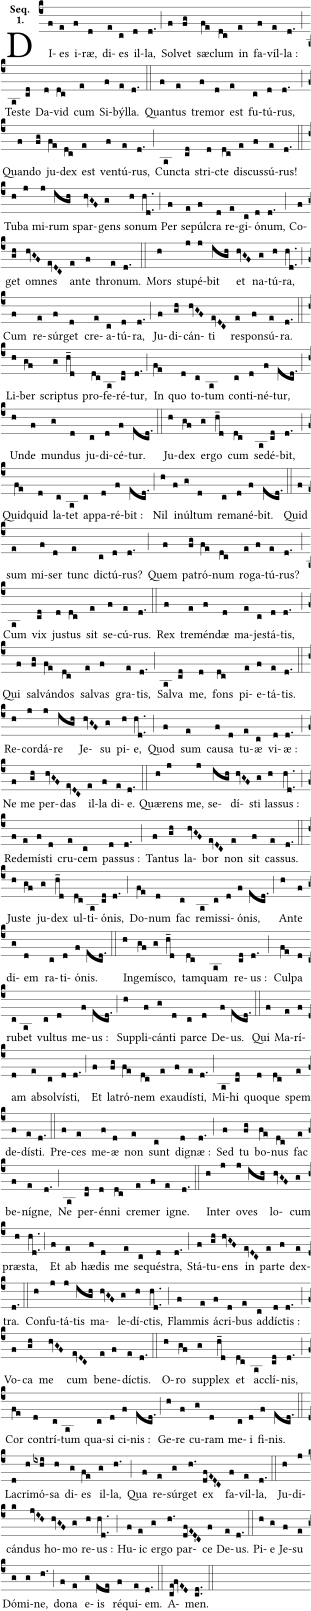
\includegraphics[width=0.75\textwidth]{figures/ud-03/dies-irae-solesmes.eps}
    \caption{Partitura do Introito «Puer natus est»}
    \label{fig:puer-natus}
\end{figure}
% -----------------------
%
%\newpage
%
% EXERCICIO 3.- Fichas audicións
%
% -----------------------------------
% FICHAS DE AUDICIÓNS PARA COMPLETAR:
% -----------------------------------
\section{Coñece a música do medievo}
%
Escoita con atención as audicións propostas para este trimestre e completa as fichas. Fai un breve resumo das principais características da obra.
Podes atopar máis info na aula virtual de Historia da Música I.
%
\begin{multicols}{2}
%
% AUDICIÓN 1.- PUER NATUS EST NOBIS
% ---------------------------------
% Exemplo de canto chá: Puer natus est nobis - Introito (Modo VII)
%
\begin{ejercicio}[Puer natus est nobis] 
%
Completa a ficha da obra proposta como exercicio de audición.
%
	\begin{enumerate}[1.-]
        \vspace*{0.3cm}
		\item
			Autor: \dotfill
			\vspace*{0.3cm}
		\item
			Obra:
			\begin{enumerate}[a)]
			    \item Título: \dotfill \vspace*{0.3cm}
			    \item Período: \dotfill \vspace*{0.3cm}
			    \item Forma: \dotfill \vspace*{0.3cm}
			    \item Timbre: \dotfill 			\vspace*{0.3cm}
			    \item Textura: \dotfill \vspace*{0.3cm}
			    \item Estilo: \dotfill \vspace*{0.3cm}
			    \item Xénero: \dotfill 
			    \vspace*{0.3cm}
			\end{enumerate}
		\item 
		    Resume as principais características que definen a obra:
			\vspace*{8.0cm}			

	\end{enumerate}
\end{ejercicio}
%
%
\begin{ejercicio}[Dies irae]
%
Completa a ficha da obra proposta como exercicio de audición.
%
	\begin{enumerate}[1.-]
        \vspace*{0.3cm}
		\item
			Autor: \dotfill
			\vspace*{0.3cm}
		\item
			Obra:
			\begin{enumerate}[a)]
			    \item Título: \dotfill \vspace*{0.3cm}
			    \item Período: \dotfill \vspace*{0.3cm}
			    \item Forma: \dotfill \vspace*{0.3cm}
			    \item Timbre: \dotfill \vspace*{0.3cm} 		
			    \item Textura: \dotfill \vspace*{0.3cm}
			    \item Estilo: \dotfill \vspace*{0.3cm}
			    \item Xénero: \dotfill \vspace*{0.3cm}
			\end{enumerate}
		\item 
		    Resume as principais características que definen a obra:
			\vspace*{8.0cm}			

	\end{enumerate}
\end{ejercicio}
%
\end{multicols}
%
%\newpage
%
\input{actividades/Exercicios/HM1-TR2-2022/Exercicio4-Can-vei-comentario.tex}
%
%\input{Exercicio5-Seikilos-comentado}
%
%%
% ----
\hideanswers % oculta respostas
%
% Cargamos os Exercicios:
\loadallproblems[Tema3-GREGO]{../../Cuestions/Tema3-Canto-gregoriano.tex}
\loadallproblems[Tema3-GREGO1]{../../Cuestions/Tema3-Canto-gregoriano-expansion.tex} %
%\loadallproblems[Tema3-NOTA]{../../Cuestions/Tema3-Notacion-modal.tex} %
%\loadallproblems[Tema1-PENS]{../../Cuestions/Tema1-Pensamento.tex} %
%\loadallproblems[Tema1-RO]{../../Cuestions/Tema1-Roma.tex} %
%\loadrandomproblems[loops]{2}{loops}% aleatorios
%
% FOLLA EXERCICIOS: 
% -----------------
\begin{multicols}{2} % a 2 columnas
    \begin{enumerate}
%\useproblem{input}
    \foreachproblem[Tema3-GREGO]{\item\label{prob:\thisproblemlabel}\thisproblem}
    \foreachproblem[Tema3-GREGO1]{\item\label{prob:\thisproblemlabel}\thisproblem}
 %   \foreachproblem[Tema3-NOTA]{\item\label{prob:\thisproblemlabel}\thisproblem}
%    \foreachproblem[Tema1-PENS]{\item\label{prob:\thisproblemlabel}\thisproblem}
    \end{enumerate}
\end{multicols}
%
% SOLUCIONS:
% ----------
%\newpage
%\begin{multicols}{2}
%\showanswers
%\begin{itemize}
%\foreachdataset{\thisdataset}{%
%\foreachproblem[\thisdataset]{\item[\ref{prob:\thisproblemlabel}]\thisproblem}
%}
%\end{itemize}
%\end{multicols}
\end{document}
%Fin de Hoja de ejercicios
%